\documentclass{article}
\usepackage{tikz}
\usetikzlibrary{shapes, positioning, fit, backgrounds, arrows.meta}

\begin{document}
\begin{figure}[htbp]
\centering
\vspace{1cm}
\resizebox{\textwidth}{!}{
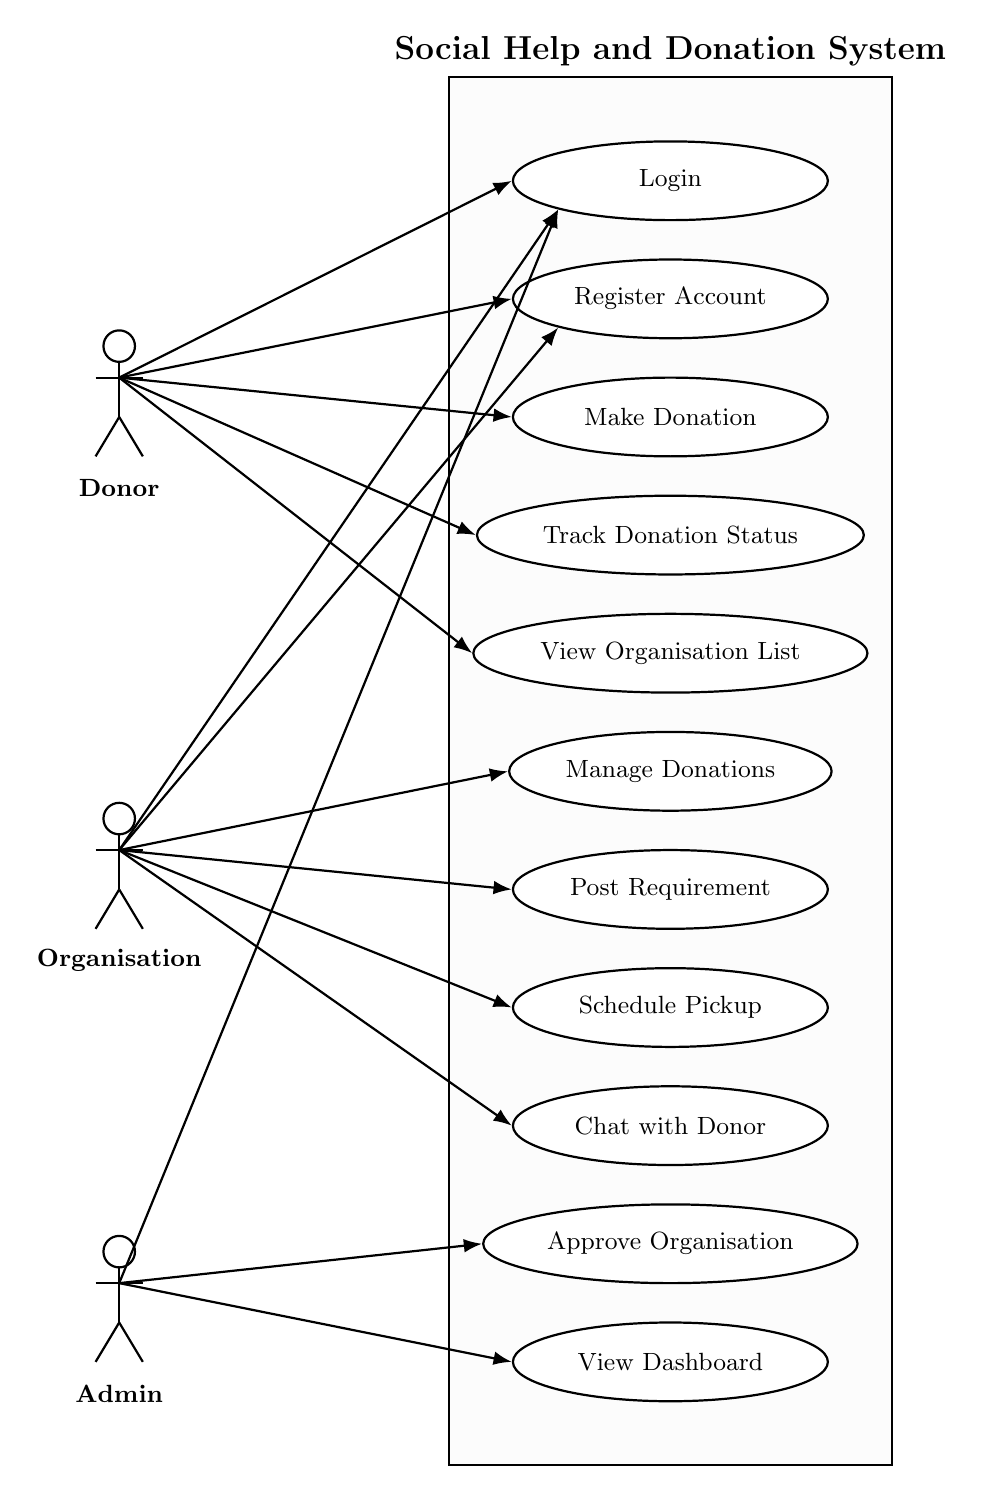
\begin{tikzpicture}[
    >=Latex, thick,
    actor/.style={align=center, font=\small\bfseries},
    usecase/.style={draw, ellipse, minimum width=4cm, minimum height=1cm, align=center, fill=white, font=\small}
]

% -------------------------
% Custom Stickman Definition
% -------------------------
\tikzset{
    stickman/.pic={
        \coordinate (-chest) at (0, 0);
        \draw[thick] (0, 0.4) circle (0.2); % Head
        \draw[thick] (0, 0.2) -- (0, -0.5); % Body
        \draw[thick] (-0.3, 0) -- (0.3, 0); % Arms
        \draw[thick] (0, -0.5) -- (-0.3, -1); % Left Leg
        \draw[thick] (0, -0.5) -- (0.3, -1); % Right Leg
    }
}

% -------------------------
% Use Cases (Center Column inside Boundary)
% -------------------------
\node[usecase] (UC1) at (0, 7.5) {Login};
\node[usecase] (UC2) at (0, 6) {Register Account};
\node[usecase] (UC3) at (0, 4.5) {Make Donation};
\node[usecase] (UC4) at (0, 3) {Track Donation Status};
\node[usecase] (UC5) at (0, 1.5) {View Organisation List};
\node[usecase] (UC6) at (0, 0) {Manage Donations};
\node[usecase] (UC7) at (0, -1.5) {Post Requirement};
\node[usecase] (UC8) at (0, -3) {Schedule Pickup};
\node[usecase] (UC9) at (0, -4.5) {Chat with Donor};
\node[usecase] (UC10) at (0, -6) {Approve Organisation};
\node[usecase] (UC11) at (0, -7.5) {View Dashboard};

% -------------------------
% System Boundary Envelope
% -------------------------
\begin{scope}[on background layer]
    \node[draw, rectangle, thick, fill=gray!2, inner sep=0.8cm, fit=(UC1) (UC11)] (System) {};
    \node[anchor=south, font=\large\bfseries] at (System.north) {Social Help and Donation System};
\end{scope}

% -------------------------
% Actors Definition
% -------------------------

% 1. Donor Actor (Top Left)
\pic (DonorPic) at (-7, 5) {stickman};
\node[actor] (DonorLabel) at (-7, 3.6) {Donor};

% 2. Organisation Actor (Middle Left)
\pic (OrgPic) at (-7, -1) {stickman};
\node[actor] (OrgLabel) at (-7, -2.4) {Organisation};

% 3. Admin Actor (Bottom Left)
\pic (AdminPic) at (-7, -6.5) {stickman};
\node[actor] (AdminLabel) at (-7, -7.9) {Admin};

% -------------------------
% Association Paths
% -------------------------

% Donor Links
\draw[->] (DonorPic-chest) -- (UC1.west);
\draw[->] (DonorPic-chest) -- (UC2.west);
\draw[->] (DonorPic-chest) -- (UC3.west);
\draw[->] (DonorPic-chest) -- (UC4.west);
\draw[->] (DonorPic-chest) -- (UC5.west);

% Organisation Links
\draw[->] (OrgPic-chest) -- (UC1.south west);
\draw[->] (OrgPic-chest) -- (UC2.south west);
\draw[->] (OrgPic-chest) -- (UC6.west);
\draw[->] (OrgPic-chest) -- (UC7.west);
\draw[->] (OrgPic-chest) -- (UC8.west);
\draw[->] (OrgPic-chest) -- (UC9.west);

% Admin Links
\draw[->] (AdminPic-chest) -- (UC1.south west);
\draw[->] (AdminPic-chest) -- (UC10.west);
\draw[->] (AdminPic-chest) -- (UC11.west);

\end{tikzpicture}
}
\caption{Use Case Diagram for Social Help and Donation System}
\end{figure}
\end{document}
